\documentclass[english,notitlepage,reprint,nofootinbib]{revtex4-1}  

\usepackage[utf8]{inputenc}


\usepackage{physics,amssymb}  % mathematical symbols (physics imports amsmath)
\include{amsmath}
\usepackage{graphicx}         % include graphics such as plots
\usepackage{xcolor}           % set colors
\usepackage{hyperref}         % automagic cross-referencing
\usepackage{listings}         % display code
\usepackage{subfigure}        % imports a lot of cool and useful figure commands
% \usepackage{float}
%\usepackage[section]{placeins}
\usepackage{algorithm}
\usepackage[noend]{algpseudocode}
\usepackage{subfigure}
\usepackage{tikz}
\usetikzlibrary{quantikz}
\hypersetup{
    colorlinks,
    linkcolor={red!50!black},
    citecolor={blue!50!black},
    urlcolor={blue!80!black}}


% ===========================================


\begin{document}

\title{}  % self-explanatory
\author{} % self-explanatory
\date{\today}                             % self-explanatory
\noaffiliation                            % ignore this, but keep it.

%This is how we create an abstract section.
\begin{abstract}
    \end{abstract}
\maketitle


% ===========================================
\section{Introduction}

%

% ===========================================
\section{Methods}\label{sec:methods}
%

% ===========================================
\subsection*{The algorithm}
%

% ===========================================
\section{Results}\label{sec:results}
%
\begin{figure}[ht]
	\centering
	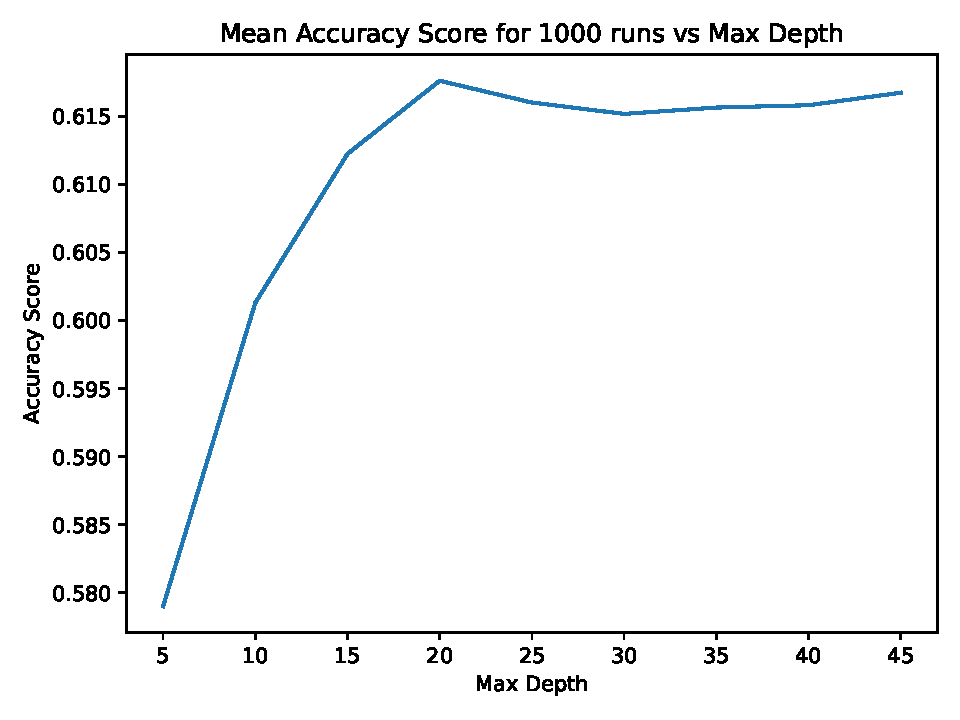
\includegraphics[width=\linewidth]{../plots/tree-accVSdepth.pdf}
	\caption{Mean accuracy score plotted against random forests with 500 trees for the given maximum depth. }
	\label{fig:accVSdepth}
\end{figure}

% ===========================================
\section{Discussion}\label{sec:discussion}
%
In order to find the optimal depth for a decision tree, we ran for depth from $ 5 $ to $ 45 $ for step size of 5 first and the result is presented in Figure~\ref{fig:accVSdepth}. We discovered that after the rapid ascend initially, the best performance was reached around maximum depth of $ 20 $. We repeat the tuning process for depth $ \in [15, 25] $, with step size of $ 2 $ and $ 1000 $ trees per forests. 

% ===========================================
\section{Conclusion}\label{sec:conclusion}

\onecolumngrid

%\bibliographystyle{apalike}
\bibliography{ref}


\end{document}
